\documentclass{article}

\usepackage[margin=2.0cm]{geometry}

\usepackage{tikz}
\usetikzlibrary{automata}
\usepackage{amsmath,amsthm,amssymb}

\newcommand{\N}{{\ensuremath \mathbb{N}}}

\newtheorem{proposition}{Proposition}

\author{Jacob Thomas Errington (260636023)}
\date{22 October 2015}
\title{Assignment \#3\\Theory of Computer -- COMP 330}

\begin{document}

\maketitle

\begin{enumerate}
    \item True or false.

        \begin{proposition}
            It is not the case that if $A$ is regular and 
            $A \subseteq B$, then $B$ must be regular.
        \end{proposition}

        \begin{proof}
            Let $A = \{a^n b^n | n \in \N\}$. Clearly, this is a subset
            of $\Sigma^*$, which is regular.
        \end{proof}

        \begin{proposition}
            It is not the case that if $B$ is regular and 
            $A \subseteq B$, then $A$ must be regular.
        \end{proposition}

        \begin{proof}
            Let $A = \{a^n b^n | n \in \N\}$ (the language containing
            only the string $ab$). Clearly, $A$ is a subset of the
            language $B = a^* b^*$.
        \end{proof}

        \begin{proposition}
            If $A$ and $AB$ are both regular then $B$ must be regular.
        \end{proposition}

        \begin{proof}
            A DFA for $AB$ can be formed from DFAs for $A$ and for $B$.
            Hence, within the DFA for $AB$, there is a DFA for $B$,
            which shows that $B$ is regular.
        \end{proof}

        \begin{proposition}
            It is not the case that if $\{A_i | i \in \N\}$ an infinite
            family of regular languages, then $\bigcup_i^\infty A_i$ is
            a regular language.
        \end{proposition}

        \begin{proof}
            Suppose the language $A_i$ is the language accepting only
            the string $a^i b^i$. Then, the infinite union of those
            languages is the language $\{ a^n b^n | n \in \N \}$.
        \end{proof}

    \item Show that the languages are not regular.

        \begin{proposition}
            The language $L = \{a^n b^m a^{n + m} | n, m \geq 0\}$ is not
            regular.
        \end{proposition}

        \begin{proof}
            We will use the pumping lemma.

            Demon picks $p$.

            I pick  $s = a^p b^p a^{2p}$.

            Demon picks $xyz = s$ such that $|xy| \leq p$ and $|y| > 0$.
            Hence, $y = a^k$.

            I pick $i = 2$, so as to make 
            $s^\prime = a^{p + k} b^p a^{2p} \notin L$.
        \end{proof}

        \begin{proposition}
            The language $\{x | x = x^R, x \in \Sigma^*\}$.
        \end{proposition}

        \begin{proof}
            We will use the pumping lemma.

            Demin picks $p$.

            I pick $s = a^p b^p$. Clearly this is a palindrome.

            Demon picks $xyz = s$ such that $|xy| \leq p$ and $|y| > 0$.
            Hence, $y = a^k$.

            I pick $i = 2$, so as to make
            $s^\prime = a^{p + k} b^p \notin L$.
        \end{proof}

    \item
        Consider the language 
        $F = \{a^i b^j c^k | i, j, k \geq 0,\, i = 1 \implies j = k\}$.

        \begin{proposition}
            The language $F$ is not regular.
        \end{proposition}

        \begin{proof}
            First we will show that $F$ is not regular, by using the pumping
            lemma. However, rather than show that $F$ is not regular, we will
            show that the reverse language is not regular.

            Demon picks $p > 0$.

            We pick $s = c^p b^p a$.

            Demon picks $xyz = s$ such that $|xy| \leq p$ and $|y| > 0$. Hence,
            $y = c^k$.

            We pick $i = 2$, so as to make 
            $s^\prime = c^{p + k} b^p a \notin L$.

            Since $F^R$ is not regular, $F$ is not regular.
        \end{proof}

        \begin{proposition}
            The language $F$ can be pumped.
        \end{proposition}

        \begin{proof}
            First, remark that pumping irregular languages does not contradict
            the pumping lemma. The pumping lemma states that if a language is
            regular, then it can be pumped, not that if it can be pumped, then
            it is regular.

            We pick $p = 2$.

            Demon picks $s \in L$ such that $|s| > p$. Since $s \in L$,
            $s = a^i b^j c^k$.

            If $s$ begins with $aal$ where $l \neq a$, then $y = aa$ and $z$ is
            the rest. Otherwise, $y$ is the first letter and $z$ is the rest.
            In either case, $x = \epsilon$.

            Demon picks $i \geq 0$, so as to form $x y^i z = y^i z$.

            First, notice that our choice of $x$, $y$, and $z$ preserves the
            relative order of the letters in the strings. It suffices to show
            now that the number of $a$s does not become $1$ after pumping
            when it was not originally so.

            If there is a single $a$ in the original string, then $y = a$, and
            pumping it will either increase the number of $a$s or make it zero,
            and such strings are in the language.

            If there are more than two $a$s in the original string, then 
            $y = a$, and pumping it cannot make the number of $a$s equal to
            $1$.

            If there are no $a$s in the original string, then $y$ is the first
            letter of the string, and changing its count has no effect on
            whether the resulting string is in the language.
        \end{proof}

    \item 
        \begin{enumerate}
            \item
                See figure \ref{fig:dfa} for a DFA for the language of words
                having an even number of $a$s, an odd number of $b$s, and not
                containing the string $ab$.

                \begin{figure}[h]
                    \caption{
                        A DFA with five states for recognizing the language of
                        words having an even number of $a$s, an odd number of
                        $b$s, and not containing the string $ab$.
                    }

                    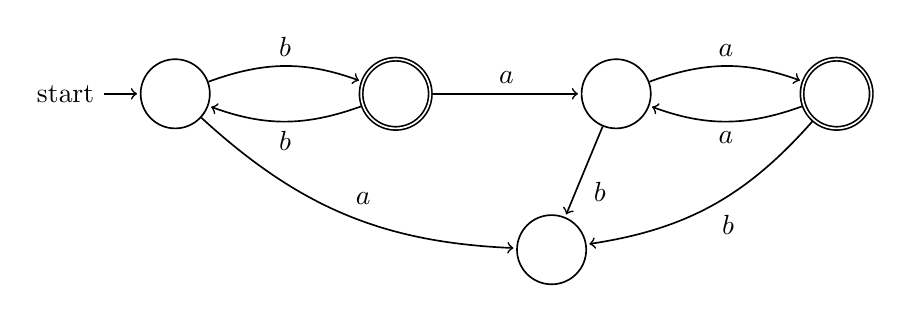
\begin{tikzpicture}[
                            ->,
                            shorten >=1pt,
                            auto,
                            node distance=2.8cm,
                            semithick
                        ]

                        \tikzstyle{every state}=[fill=white,draw=black,text=black]

                        \node[initial,state]   (A) {} ;
                        \node[accepting,state] (B) [right of=A] {} ;
                        \node[state]           (C) [right of=B] {} ;
                        \node[accepting,state] (D) [right of=C] {} ;
                        \node[state]           (E) [below right of=B] {};

                        \path
                        (A) edge [bend left=20]  node {$b$} (B)
                        (A) edge [bend right=20] node {$a$} (E)
                        (B) edge [bend left=20]  node {$b$} (A)
                        (B) edge                 node {$a$} (C)
                        (C) edge [bend left=20]  node {$a$} (D)
                        (D) edge [bend left=20]  node {$a$} (C)
                        (C) edge                 node {$b$} (E)
                        (D) edge [bend left=20]  node {$b$} (E)
                        ;
                    \end{tikzpicture}

                    \label{fig:dfa}
                \end{figure}

            \item A regular expression for this language is $b(bb)*(aa)*$.

        \end{enumerate}

    \item
        Considering the language $L = \{a^n b^m | n \neq m\}$, which is not
        regular, we wish to explicitly identify infinitely many distinct
        equivalence classes on its relation $\equiv_L$.

        First, notice that if $x \not \equiv_L y$ then
        $$
        \exists z :
        (xz \in L \land yz \notin L) \lor (xz \notin L \land yz \in L)
        $$

        We will look at strings of the form $a^{2i} b^i$. We will show that
        strings made by a choice of $i$ are not equivalent to strings made by
        the choice $j < i$. To do so, we must construct an appropriate $z$ in
        the following statement.

        $$
        \exists z:
        a^{2j} b^{j} z \notin L \land a^{2i} b^i z \in L
        $$

        We simply choose $z = b^j$.

        The left hand side will have matching numbers of $a$s and $b$s, so it
        is not in the language. The right hand side will be in the language,
        however, since $2i > i + j$

        Hence each choice of $i$ identifies a different equivalence class.
\end{enumerate}

\end{document}
